\documentclass[twocolumn]{article}

\usepackage[unicode=true, hidelinks]{hyperref}
\usepackage{enumitem}
\usepackage{graphicx,grffile}
\usepackage{xcolor}
\hypersetup{
	colorlinks,
	linkcolor={red!50!black},
	citecolor={blue!50!black},
	urlcolor={blue!80!black}
}

\title{\textbf{Autoreduction - an automated data reduction system for beamline instruments at the ISIS Facility}}
\author{J. R. Corderoy, T. Gowland, L. Greenwood, M. Noble, D. Oram and A. J. Markvardsen \\
(code contributors)\\
ISIS Facility, Rutherford Appleton Laboratory\\
Email: someone with an STFC email account}
\date{23/09/2015}

\begin{document}
\maketitle

\subsection*{Abstract}\label{abstract}

A key step for users of large research facilities is the
processing of instrument data before use. Autoreduction is a software
system designed to automate this process, integrate with other
pre-existing facility systems and software packages, and provide
an interface for users to control it.

This article describes the system setup for Autoreduction at the ISIS Facility;
its motivation and design, its use and interface and its current status in production at ISIS.

\section{Introduction}\label{introduction}

Large scale research facilities, such as the ISIS Neutron and Muon
Facility, allow users in academic and industrial research
to perform experiments using instruments set up to probe the inner 
structure and dynamics of materials. 
Common to most instruments is the need to process -- 
`reduce' -- raw data collected from an instrument into a form
that users can interprete or do further analysis on. For example
by removing instrument specific artifacts from the measured data, 
transforming the data into different units and/or
into data formats readable by further analysis software.

The purpose of the autoreduction system is to provide a useful automation
step in this process. The system described in this paper allows data coming 
off an instrument to be automatically reduced using a dedicated software package 
such as Mantid \cite{mantid}, whilst also lending transparency to the process and
letting users control it through a straightforward web interface.

Automated data reduction is a concept which is actively persued at other large facilities.
At the NOBUGS 2016 Conference \cite{NOBUGS}, there were several talks given by delegates
from other large scale facilities which mentioned the automated reduction of data at a variety
of facilities. 

Data Analysis Infrastructure for DLS MX/CX \cite{dls-talk} discusses a batch
script based system for macromolecular beamlines. It makes use of ActiveMQ \cite{activemq}
(which will be discussed later in this paper) and also has a front end status monitor to
show the health of the system during run-time. Integration of Fast Detectors 
into Beamline Control \cite{anl-talk} also mentioned the use of automatic data processing.
To keep up with the data rates from faster detectors, they are now automatically reducing data
immediately so that users can see the results as soon as the dataset is taken.

\section{Background}\label{background}

The autoreduction system at ISIS was inspired by an autoreduction setup at the
the Spallation Neutron Source (SNS) at Oak Ridge National Laboratory \cite{autoreduceSNS}. 

The autoreduction implementation at ISIS uses the same underlying 
technologies (choice of programming language and queue node software
for example) as those used for the implementation of the SNS autoreduction
service. However, the ISIS implementation differs in that its front end 
client is designed to serve autoreduction users only and was not orginally 
part of the SNS implementation.

\subsection{Data reduction}\label{data-reduction}

The autoreduction service exists to reduce beamline instrument data. An
instrument produces discrete tranches of data, referred to as `runs', in
service of experiments. This raw data typically needs to be processed --
`reduced' -- before it can be used by scientists. This is done by running a 
script on it. Although the script itself need not change often, it may have
configurable parameters -- variables -- which might require more frequent
updating.

The autoreduction system is intended to automate this process.
Instrument scientists provide the system with reduction scripts - in a specified
location on a shared file archive - along with sets of variables to use to
reduce runs. Firstly, the system watches  for the completion of runs. Once a new
completed run has been found, the system will then run the appropriate script
with the correct variables on the new run. Once the script has finished execution,
reduced data will be saved to a data store for users to retrieve.

\subsection{Requirements}\label{requirements}

The system is intended to serve the instrument scientists (who manage beamline instruments) 
and users who use the instruments to run experiments. 
The key requirements from these users, which have been completed to date, are:

\begin{enumerate}[noitemsep]
\item
  Automate the reduction of data from beam instruments, using scripts
  provided by instrument scientists
\item
  Show the status of reduction on runs, as well as the results and
  locations of reduced data, to users
\item
  Allow instrument scientists to set the parameters used for reduction
  in advance of experiments and optionally schedule these to be diffirent
  for particular experiment
\item
  Allow users and instrument scientists to see what script and with which
  parameters was used to reduce a run
\item
  Allow users and instrument scientists to modify the parameters used
  for a run and re-run reduction using new parameters or scripts
\end{enumerate}

Additional constraints are:

\begin{enumerate}[noitemsep]
\item
  Limit access to the system to ensure that only staff and scientists
  can access runs and instruments
\item
  Utilise existing authentication systems to validate identities and
  permissions for (1)
\item
  Allow scalability for processing large amounts of data in a timely
  manner
\end{enumerate}

\section{System architecture}\label{system-architecture}

The architecture is based on a queue node which co-ordinates
communication between all components of the system. This maintains
separate message queues which allow components to act on messages from
other components and update the system. These components are:

\begin{itemize}[noitemsep]
\item
  A monitor for new instrument runs
\item
  The state database \& coordinator
\item
  A worker for reduction processing
\end{itemize}

When the monitor detects that a new run has completed on an instrument, it will send a 
message to the \emph{Data Ready} queue. The \emph{QueueProcessor} process will consume this
message, strip out the relevant information and creates a corresponding job in the database.
\emph{QueueProcessor} will then send the message on to the \emph{Reduction Pending} queue.
The \emph{AutoreductionProcessor} process will be watching the \emph{Reduction Pending} queue.
When \emph{AutoreductionProcessor} recieves a message, it runs the \emph{PostProcessAdmin} 
script which will send a message to the \emph{ReductionStarted} queue such that the database
remains up to date. Once reduction has finished, \emph{PostProcessAdmin}  will send the
result to either \emph{Reduction Complete} or \emph{Reduction Error} where it will be consumed
by the \emph{QueueProcessor} and updated in the database.


\begin{figure*}
\centering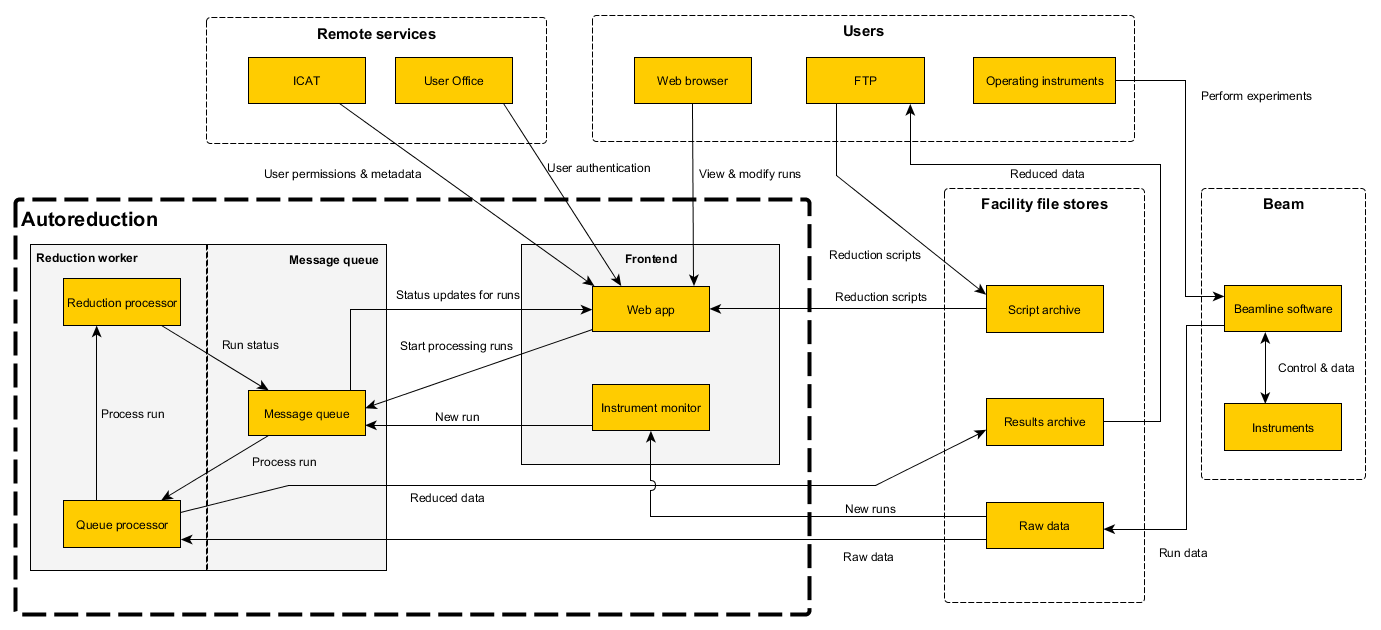
\includegraphics[width=1.15\linewidth,angle=90,origin=c]{system.png}
\caption{How the current autoreduction system fits into the ISIS workflow.}
\end{figure*}

\subsection{Message queue}\label{message-queue}

Apache ActiveMQ \cite{activemq} is used as the message queueing system using 
JSON-formatted objects as messages. The intention of the message
is conveyed by which queue it's placed in rather than a field in the
message itself. Runs can be `scheduled' simply by using ActiveMQ's
scheduled delay feature which allows a message to be delivered a given
time after it's been pushed to the queue.

Messages contain metadata for the run such as a (unique) run number and
version, the experiment and instrument that the data is associated with,
and any logs or errors resulting from reduction. They also carry the
necessary information to carry out the data reduction - the Python
script to run on the data, paths to the data, and variables to be used
by the script.

Data files at ISIS typically run in the hundreds of MB. They are therefore 
impractical to be sent directly in a message and instead they're provided as file
paths on a shared file archive. Meanwhile, the reduction script to be
used is sent as a string; the script is served from the state database
and using the message queue to directly send it obviates the need to
rely on a potentially flaky shared file store within the system.

\subsection{Run monitor}\label{run-monitor}

When a new run has been completed on the beam line, the raw data files are
placed in a shared filesystem. A node runs a Python watchdog daemon that
tracks changes in this filesystem and, when a new run is detected, will send a
message to \emph{Data Ready} with details of the run. The particular
choice of monitor isn't crucial; anything would work as long as it
pushed the same message to the queue. In the current production system
at ISIS, the run monitor is on same node as the state database itself.

\subsection{State database \& coordinator}\label{state-database}

The \emph{QueueProcessor} service runs as a daemon and is the service responsible
for keeping track of the status of jobs in an SQL database. The service
listens on the \emph{Data Ready} queue. When messages are first received,
the service will set the correct variables for the job, create new jobs in 
the database and, when ready, will send a message to the \emph{Reduction Pending} queue.

The daemon service also receives updates from the reduction worker itself. When the 
reduction worker reaches certain stages of its execution, it will send messages to
\emph{Reduction Started}, \emph{Reduction Complete} and \emph{Reduction Error}.
The \emph{QueueProcessor} service also listens on these queues and will update the database
accordingly when messages are received. For some messages in the error queue, the daemon 
will create and schedule the appropriate retry runs. There is also a system in place for 
emailing notifications of run failures to administrators. 

Since the database is being frequently being updated throughout the process of autoreduction,
the Python/Django\cite{django} WebApp is always up to date with the latest information.
This means that users can easily check on the progress of their runs and get a good idea of 
how long it is going to take for them to retrieve their data at the end.

\subsection{Reduction worker}\label{reduction-worker}

The data reduction itself is performed by a worker node, running a
Python daemon listening on \emph{Reduction Pending}. When the worker
consumes a message, it will spawn a process starting the job and
notifying \emph{Reduction Started}. This process tests for access to the
filesystems used for storing the raw and reduced data, triggering a
scheduled retry later -- on \emph{Reduction Error} -- if they're
unavailable. Otherwise, it will proceed with the reduction, loading and
then running the provided reduction script.

On a successful execution, the daemon will notify \emph{Reduction Completed} with
the location of the reduced data; otherwise, it will send the reason for
failure to \emph{Reduction Error}, most likely without triggering a
retry. In both cases, it will create logs of the process and also clean up
after itself. Some runs associated with the same experiment will write
output to the same directory; to prevent clashes due to this, the node
contains an internal queue holding all jobs associated with a given
experiment for as long as it is actively reducing runs for the
same experiment.


\begin{figure*}
\centering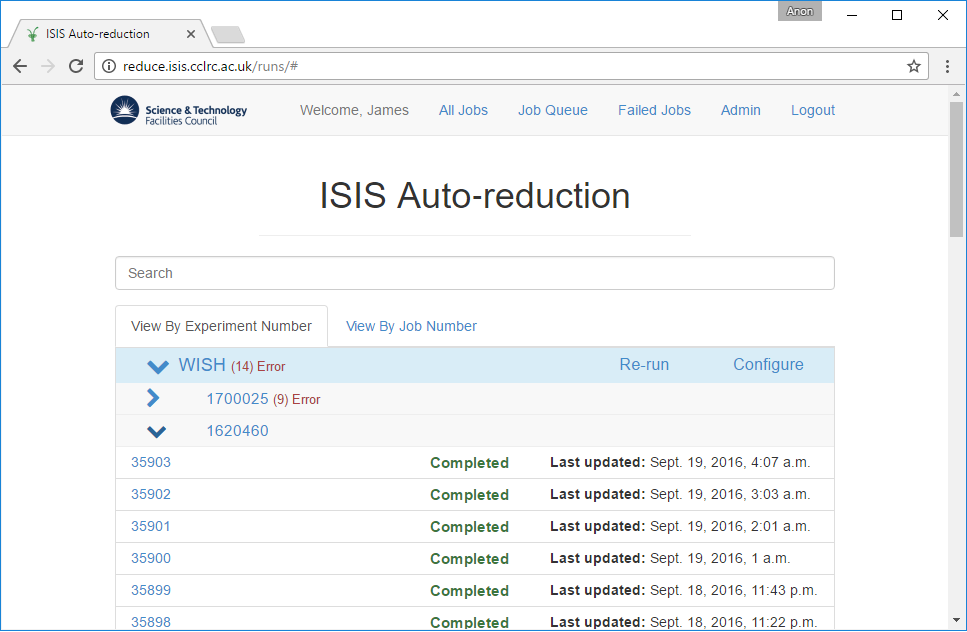
\includegraphics[width=0.8\linewidth]{index.png}
\caption{The web app index, showing recent runs.}
\end{figure*}

\section{Interface}\label{interface}

\subsection{Reduction scripts}\label{reduction-scripts}

The wholly automated portion of the system revolves around running
scientist-provided scripts to reduce raw instrument data. These scripts
are provided as Python scripts on a per-instrument basis, typically
using the Mantid software package to do the heavy lifting. They're
stored on a shared file store in a known location where they can be
modified at will by instrument scientists. The script used in
reduction is also stored in the system database.

Aside from overall logic, these scripts typically require parameters
such as calibration files, information about how the instrument was run,
output settings, and so on. A mechanism for providing such parameters 
separate from the script itself is provided. A list of parameters and
default values is provided in a Python file similar to the reduction
script. The autoreduction system keeps track of the parameter
configurations provided to it and applies them to the relevant jobs.

The scripts need to integrate with the automation system, and
as such must conform to a certain specification: a reduction script must have a
\emph{main()} method, taking an input data file and an output directory as
arguments. If the script uses system-supplied parameters, it must have a
certain \emph{import} directive which serves as a point of injection
for the variables when the reduction script is executed.

A reduction script is a Python script and it can call any software 
callable from Python installed on the reduction worker compute nodes which
includes Mantid data reduction algorithms.

Each experiment at ISIS has a unique so-called RB-number
and for almost all experiments at ISIS multiple separate runs are collected.
A reduction script has access to all reduced data for an experiment, which 
may be used in a script to automatically combine information from multiple 
data reductions.

\subsection{Web app}\label{web-app}

The web app provides the user-facing interface for managing reduction.
It was developed in Python, using the Django web framework, and is
integrated with the state database. Django provides an intuitive way to
interact with databases through its use of models and Object Relational Mapping (ORM).
Therefore, getting information from the database to show on the front end is 
quick and intuitive. 

Users log in via the ISIS User Office system -- using credentials 
granted for facility-wide use -- and their level of access is then 
governed by ICAT's \cite{icat} information on the experiments and instruments they 
should be able to see. A searchable index of the runs is displayed on the front page, sorted
by instrument, experiment (RB-number) and/or run number, showing their reduction
status.

Each run has its own summary page with detailed information; a user can
see the status of the reduction, where the reduced data is, and the
script and variables that were used to reduce it. From here the run can
be re-run, with or without modifying the variables used and with the choice
of whether or not to overwrite the previous run's data. Any
experimenter can access this page for their runs, and it is intended that
external scientists running experiments would be able to control their data
reduction directly in this way.

Experiments also have summary pages, showing all of the runs that are
associated with a given experiment along with their status and data
locations. Metadata about the experiment is retrieved from ICAT and
displayed here.

Instrument scientists can access a summary page for their instruments,
showing the current status of runs on an instrument, as well as current
and upcoming run variables. From here, instrument scientists can assign
sets of variables by experiment and run number which will then be used
for new runs. Batch re-running of past jobs is also possible here. 
This option allows instrument scientists the convenience of re-running multiple 
failed jobs should this be required. 

Administrators can access everything above and additionally have access
to pages displaying all queued and failed jobs. These pages provide an
overview of the status of the system at a glance and have controls for
batch operations on failed jobs such as to re-run them.

\section{Deployment}\label{deployment}

The system is deployed at ISIS. The node managing
the state and web app is a Windows Server system running on a 
Hyper-V\cite{hyper-v} virtualisation cluster; it serves the web app using
Microsoft's Internet Information Services (IIS)\cite{iis} and 
FastCGI\cite{fcgi}. The web app is currently only accessible from inside
the laboratory using the URL: http://reduce.isis.cclrc.ac.uk. 

There is one reduction node, running Red Hat Enterprise Linux 7\cite{rhel}
on a dedicated server -- reducing large amounts of data is memory and CPU-intensive.
This node also serves the message queue; subsequent worker nodes would
not have multiple message queues, and the message queue will be hosted
on a separate node.

The software written as part this project is not tied to a
particular operating system since it is written entirely in Python and Django. 

\section{Future plans}\label{future-plans}

It is planned that the autoreduction system be developed to further meet
the needs of users. Future development to this will involve:

\begin{enumerate}
\item
  Expanding the system to accommodate greater volume of use -- this
  might involve accomodating more reduction workers, for example
\item
  Integrating other methods of monitoring or listening for new runs -- the current
  method of watching a file archive is specific to ISIS
\item
  Make the web app to be accessible from outside of the laboratory
\item
  Have selected reduced data automatically cataloqued in ICAT 
\item
  Improving portability and deployability of the current software; the
  state database/webapp is currently somewhat nontrivial to deploy
\end{enumerate}

Longer term, the system may be extended to listen to live streams and starts
processing such data as they come off beamlines rather then waiting for files 
to be written to disk. 

\section{Conclusion}\label{conclusion}

The autoreduction system offers a convenient way of automating data reduction
on beamline instruments. It uses a scalable architecture to allow prompt
reduction of data from a large number of instruments, and utilises a web app
frontend to allow users to control the reduction process manually and verify
that the correct reduction was executed.

The source code can be found on GitHub\cite{source}.

\section{Acknowledgement}\label{Acknowledgement}

Tom Griffin, Nick Draper, Martyn Gigg, Alex Buts, other excitation group members and other testers, Shelly Ren and Mathieu Doucet.

\begin{thebibliography}{99}
\bibitem{mantid}
    O. Arnold, et al.,
    \emph{Mantid -- Data analysis and visualization package for neutron scattering and $\mu$SR experiments},
    Nuclear Instruments and Methods in Physics Research Section A, Volume 764, 11 November 2014, Pages 156-166,
    \href{http://dx.doi.org/10.1016/j.nima.2014.07.029}{10.1016/j.nima.2014.07.029}.

\bibitem{autoreduceSNS}
    G. Shipman, et al.,
    \emph{Accelerating Data Acquisition, Reduction, and Analysis at the Spallation Neutron Source},
    2014 IEEE 10th International Conference on eScience, Volume 2, 11 November 2014, Pages 224-230,
    \href{http://dx.doi.org/10.1109/eScience.2014.31}{10.1109/eScience.2014.31}.
    
\bibitem{icat}
    The ICAT Collaboration,
    \emph{The Icat Project.},
    2014,
    \href{https://doi.org/10.5286/SOFTWARE/ICAT}{10.5286/software/icat}.
    
\bibitem{activemq}
    Apache Software Foundation,
    \emph{Apache Activemq},
    \url{http://activemq.apache.org/}.

\bibitem{dls-talk}
	M. Gerstel, R. Gildea, K. Levik, A. Ashton, G. Winter.
	\emph{Data Analysis Infrastructure for DLS MX/CX},
	NOBUGS Conference 2016, Københavns Universitet,
	\url{https://indico.esss.lu.se/event/357/session/7/contribution/51/material/slides/0.pdf}

\bibitem{anl-talk}
	Dr. Sergey Stepanov.
	\emph{Integration of fast detectors into beamline controls at the GM/CA macromolecular crystallography beamlines at the Advanced Photon Source},
	NOBUGS Conference 2016, Københavns Universitet,
	\url{https://indico.esss.lu.se/event/357/session/6/contribution/17/material/slides/0.pdf}

\bibitem{NOBUGS}
	NOBUGS Conference 2016,
	\emph{NOBUGS},
	\url{https://indico.esss.lu.se/event/357/}.
    
\bibitem{django}
    Django Software Foundation,
    \emph{Django},
    \url{https://www.djangoproject.com/}.
    
\bibitem{hyper-v}
    Microsoft Corporation,
    \emph{Hyper-V},
    \url{https://technet.microsoft.com/en-us/library/mt169373.aspx}.
    
\bibitem{iis}
    Microsoft Corporation,
    \emph{IIS},
    \url{http://www.iis.net/}.
    
\bibitem{fcgi}
    \emph{FastCGI},
    \url{https://github.com/FastCGI-Archives/FastCGI.com}.
    
\bibitem{rhel}
    Red Hat, Inc,
    \emph{Red Hat Enterprise Linux},
    \url{https://www.redhat.com/en/technologies/linux-platforms/enterprise-linux}.
    
\bibitem{source}
    \emph{Autoreduction repository},
    \url{https://github.com/mantidproject/autoreduce}.

    
\end{thebibliography}
\end{document}
